We've repeated the simulation for the \emph{sequential search} problem
as did during the class. We want to study the mean of checks performed
by the sequential search algorithm before the desired element is found
in the given permutation. After we compare the mean of checks obtained
by simulation with the theoretical mean value for the same input
dimension.

The sequential search algorithm cited above is a very simple searching
method: it consume a permutation of integer of a fixed dimension $n$
and a target integer; produce true if the target belongs to the given
permutation, else otherwise (in our case we augment the information
returned with the number of checks needed in the run). The searching
strategy consists of starting from the very left and moving one step
to right every time the target is missed.

\section{Implementation}

We don't report here the description for the implementation of the
sequential search algorithm because is very simple. Instead, we focus
the explanation on the main simulation procedure.

The simulation function consume three parameters:
\begin{itemize}
\item $numdimensions$, the number of dimensions that we would like to
  test;
\item $interval$, the multiplier to build the permutation vector to be
  used during the search;
\item $attempts$, the number of application of the sequential search
  algorithm to a given permutation.
\end{itemize}
We use the number of dimensions $numdimensions$ to build a vector
$dimensions$ such that both of the following hold:
\begin{displaymath}
  \begin{split}
    length(dimensions)&=numdimensions \\
    dimensions[i]&=i * interval \quad \forall i \in \{1,\ldots,numdimensions\}
  \end{split}
\end{displaymath}
For a given dimension $n \in \{interval, 2*interval,
\ldots,numdimensions*interval\}$, we sample a permutation of integers
from $\{1,\ldots,n\}$ using the uniform distribution. For each
permutation we apply the sequential search algorithm: the number of
application is proportional to $n$ (specifically $2n$) and after every
application we record the number of checks needed to hit the target.
When we run out all the iterations we compute the mean and the
variance of the checks, storing them into auxiliary vectors.

\section{Results}

In \autoref{tab:sequential-search-table-result} we report a summary
table for a simulation invoked with arguments $numdimensions=50,
interval=20, attempts=50$. Observing the table we can see that the
simulation is quite correct, the theoretical values matches the
simulated ones with little differences.
\begin{table}[ht]
  \caption{Sequential search summary}
  \label{tab:sequential-search-table-result}
  \begin{center}
    \rotatebox{90}{
      \begin{tabular}{rrrrrrrrrr}
        \hline
        & dimensions & theo means & means & theo vars & vars
        & theo var of vars & var of vars & stand. means & stand. vars \\ 
        \hline
        1 & 20.00 & 10.50 & 10.66 & 33.25 & 34.34 & 877.80 & 975.55 & 1.22 & 1.64 \\ 
        2 & 40.00 & 20.50 & 20.65 & 133.25 & 135.02 & 14177.80 & 14994.21 & 0.82 & 0.94 \\ 
        3 & 60.00 & 30.50 & 30.48 & 299.92 & 302.46 & 71900.02 & 74572.74 & -0.10 & 0.74 \\ 
        4 & 80.00 & 40.50 & 41.09 & 533.25 & 531.28 & 227377.80 & 221994.03 & 2.28 & -0.37 \\ 
        5 & 100.00 & 50.50 & 50.52 & 833.25 & 833.01 & 555277.80 & 553196.84 & 0.07 & -0.03 \\ 
        6 & 120.00 & 60.50 & 60.13 & 1199.92 & 1189.70 & 1151600.02 & 1122368.13 & -1.18 & -1.04 \\ 
        7 & 140.00 & 70.50 & 70.42 & 1633.25 & 1621.51 & 2133677.80 & 2078575.00 & -0.22 & -0.95 \\ 
        8 & 160.00 & 80.50 & 79.80 & 2133.25 & 2155.97 & 3640177.80 & 3782358.53 & -1.92 & 1.51 \\ 
        9 & 180.00 & 90.50 & 91.06 & 2699.92 & 2696.73 & 5831100.02 & 5837985.82 & 1.44 & -0.18 \\ 
        10 & 200.00 & 100.50 & 100.26 & 3333.25 & 3315.86 & 8887777.80 & 8760281.48 & -0.59 & -0.82 \\
        ... &  &  & &  & & & &  &  \\ 
        41 & 820.00 & 410.50 & 409.84 & 56033.25 & 56005.31 & 2511768877.80 & 2520823155.84 & -0.80 & -0.16 \\ 
        42 & 840.00 & 420.50 & 419.93 & 58799.92 & 59131.53 & 2765932400.02 & 2833053962.68 & -0.68 & 1.83 \\ 
        43 & 860.00 & 430.50 & 429.49 & 61633.25 & 61801.47 & 3038913677.80 & 3061925029.95 & -1.20 & 0.89 \\ 
        44 & 880.00 & 440.50 & 441.59 & 64533.25 & 64686.44 & 3331619377.80 & 3349812105.46 & 1.27 & 0.79 \\ 
        45 & 900.00 & 450.50 & 448.81 & 67499.92 & 67476.72 & 3644977500.02 & 3620068539.03 & -1.95 & -0.12 \\ 
        46 & 920.00 & 460.50 & 461.97 & 70533.25 & 70360.59 & 3979937377.80 & 3963315767.79 & 1.68 & -0.83 \\ 
        47 & 940.00 & 470.50 & 470.75 & 73633.25 & 73791.33 & 4337469677.80 & 4381479940.27 & 0.28 & 0.74 \\ 
        48 & 960.00 & 480.50 & 481.49 & 76799.92 & 76684.82 & 4718566400.02 & 4704539498.17 & 1.11 & -0.52 \\ 
        49 & 980.00 & 490.50 & 490.41 & 80033.25 & 80176.91 & 5124240877.80 & 5142289190.74 & -0.10 & 0.63 \\ 
        50 & 1000.00 & 500.50 & 500.43 & 83333.25 & 83210.10 & 5555527777.80 & 5524755813.88 & -0.08 & -0.52 \\ 
        \hline
      \end{tabular}
    }
  \end{center}
\end{table}

We've used the standardized means to plot them against the normal
distribution in order to verify the Central Limit Theorem in
\autoref{fig:sequential-search-standardized-means}. The dotted curve
represent the normal distribution, the blue one represent the sampling
means distribution instead. Observing the plot we can say that the
approximation is quite good, however the max dimension is $n=50$, this
allow us to apply the theorem but we could gain precision if we'll
repeat our simulation for a greater value of $n$.
\begin{figure}[htb]
\centering
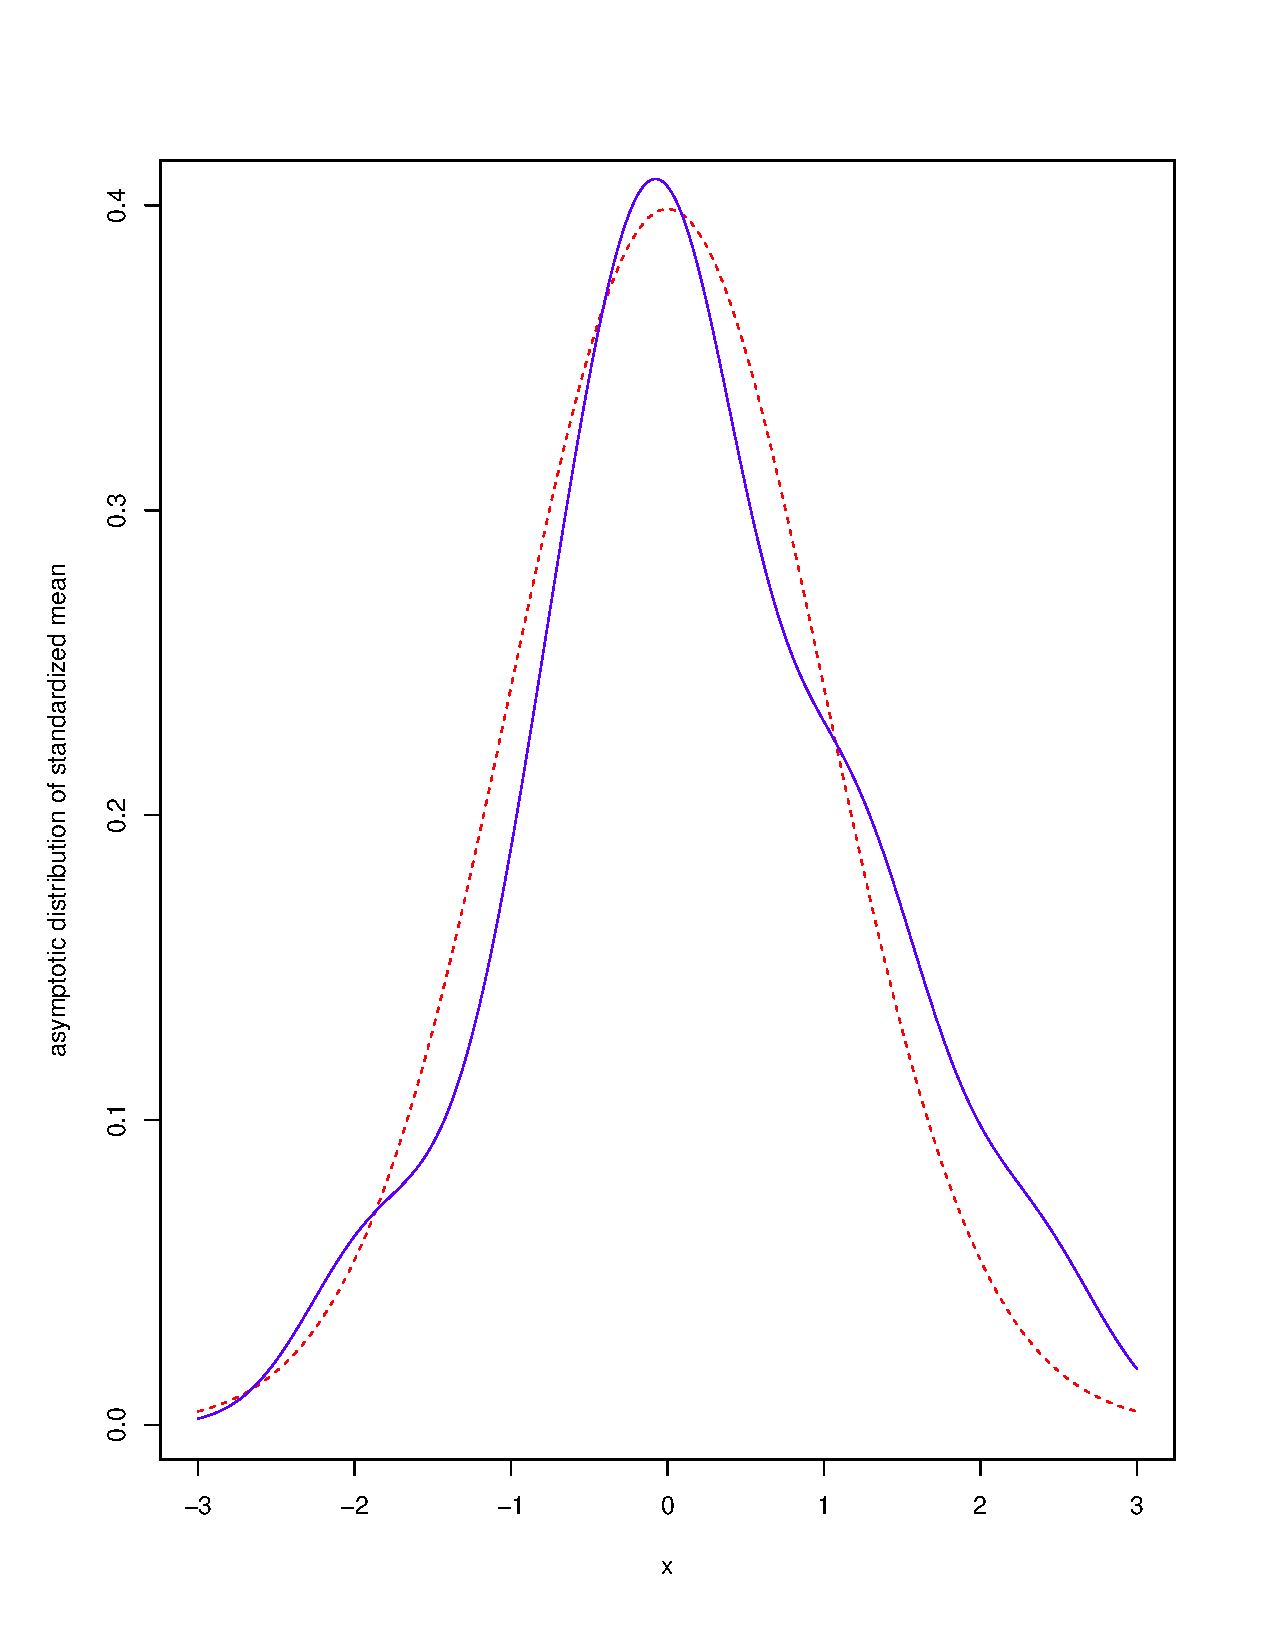
\includegraphics[height=13cm,width=13cm]{pictures/sequential-search-asymtotic-behaviour-of-standardized-means.pdf}
\caption{Plot of standardized means}
\label{fig:sequential-search-standardized-means}
\end{figure}

Also we've build a second plot with a regression of the sampling means in
\autoref{fig:sequential-search-means-regression}. The red line is
drawn after computing the intercept and the coefficient using an
hybrid model. Our attempt to explain the data consists of a mixture up
to the second degree, as follow:
\begin{displaymath}
  \begin{split}
    dims &= \sum_{i}^{n}{dimensions[i]}\\
    means &= \sum_{i}^{n}{mean[i]}\\
    dim\_squares &= \sum_{i}^{n}{dimensions[i]^2}\\
    mean\_squares &= \sum_{i}^{n}{means[i]^2}\\
    dim\_mean &= \sum_{i}^{n}{means[i] * dimensions[i]}\\
    intercept &= \frac{dim\_squares * means - dims *
      dim\_mean}{n*dim\_squares - dims^2}\\
    coefficient &= \frac{n * dim\_mean - dims * means} {n*dim\_squares-dims^2}
  \end{split}
\end{displaymath}
where $n$ is our $numdimensions$ cited above, hence the red line is
defined as $means = coefficient*dimensions + intercept$. Using an R
interpreter we can see our numerical output:
\begin{lstlisting}
  coefficient = 0.49, intercept = 0.66
  square of correlation index = 0.999
\end{lstlisting}
The regression is almost perfect, hence there exists a strong linear
relation between means and distribution (from a statistical point of
view we can conclude with the following observation: for an increment
of the dimensions of one unit we get an increment of about a half unit
on the number of checks).
\begin{figure}[htb]
\centering
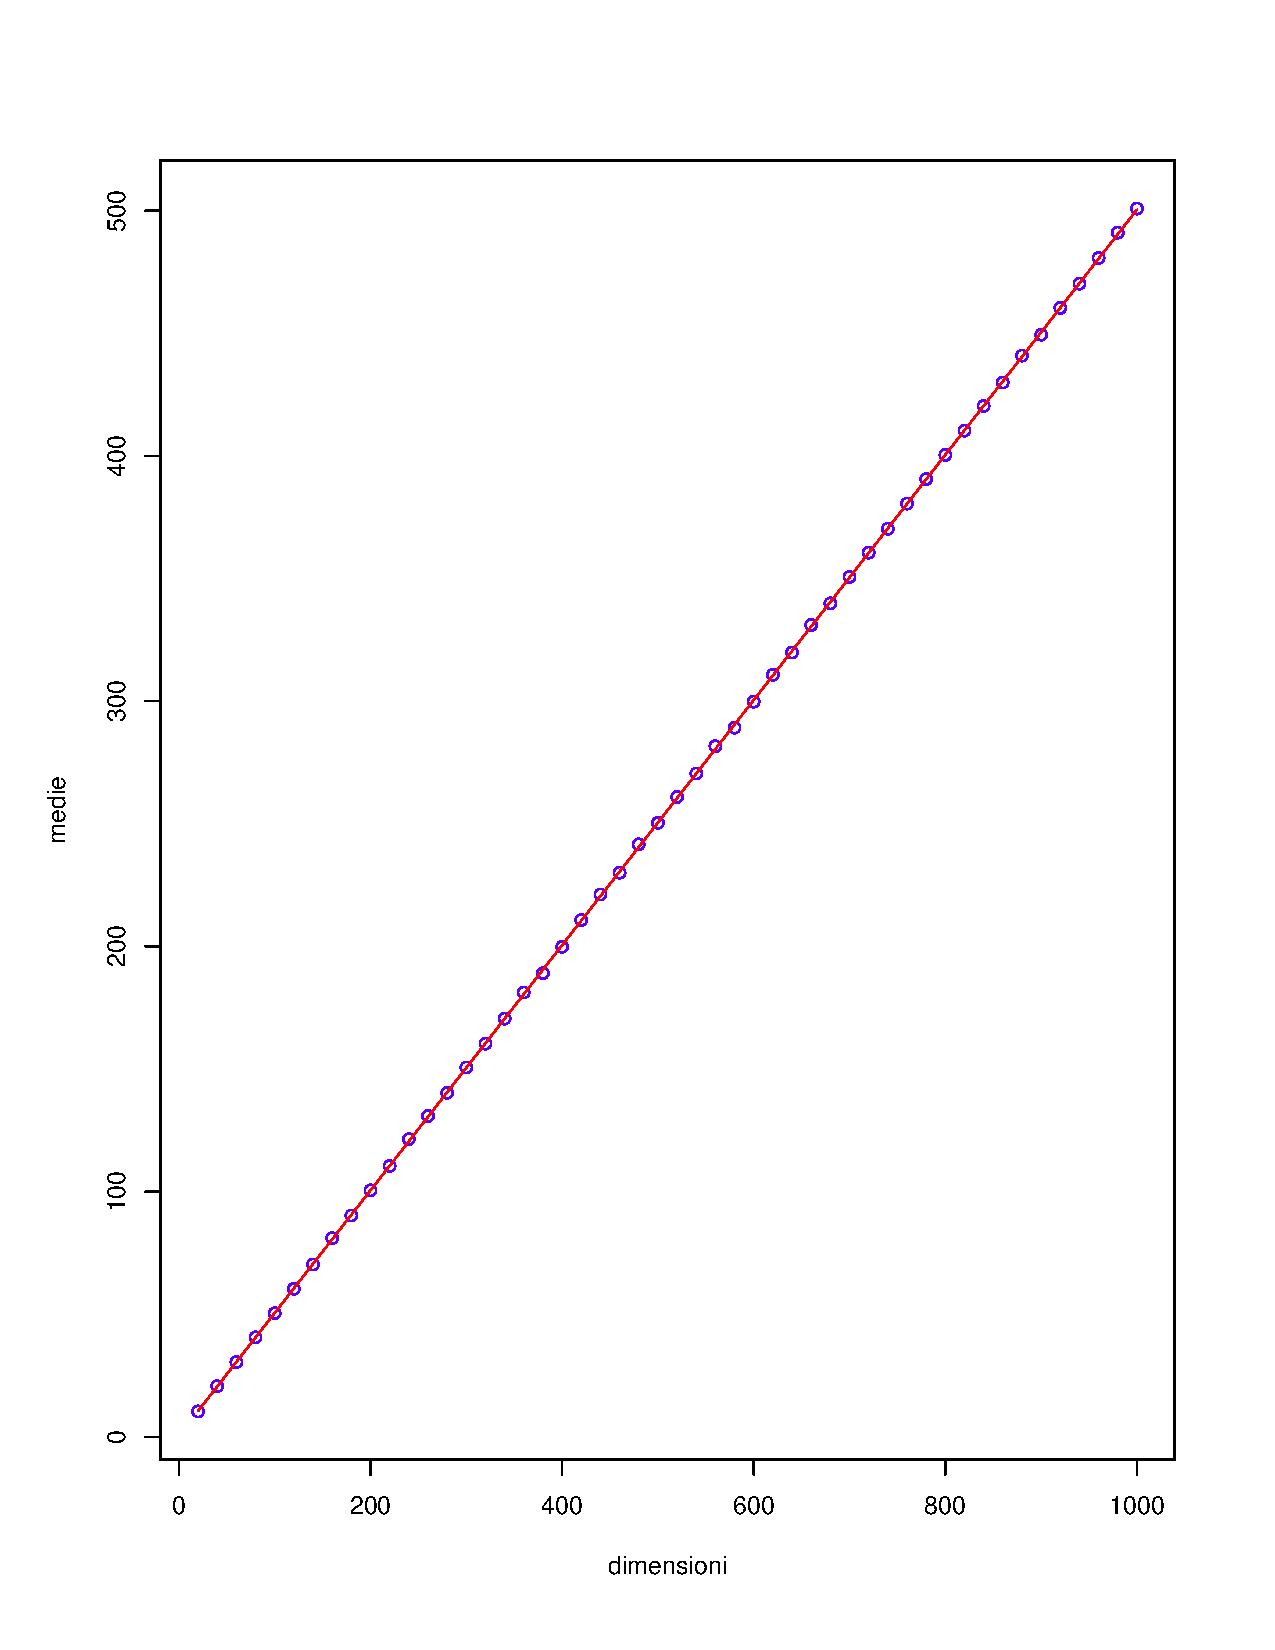
\includegraphics[height=13cm,width=13cm]{pictures/sequential-search-mean-regression-of-sequential-search.pdf}
\caption{Plot of means regression}
\label{fig:sequential-search-means-regression}
\end{figure}
